\section{灾前大气环境特征与泥石流关联因素分析}
\subsection{候选物理因素与特征量化方法}
围绕题设“冰崩—碎屑流—泥石流—山洪”灾害链，以MET、RADM、SOIL、FLUX四类塔站小时观测为主体，结合源区邻域ERA5-Land资料，分析近地层结构、天气过程和极端性。参考单事件气象过程与源区/轨迹分离研究\cite{Srivastava2022,Zhong2025}，预先定义10个因素组、14类指标、31列特征（本站18列、源区13列），而非按数据文件分节或直接指定五个因素。完整31列公式、单位、窗口、质量规则随代码字典交付。

\begin{table}[H]\centering\small
\caption{预先定义的因素组与指标家族；同组不同位置、窗口共同校准。}
\begin{tabularx}{\linewidth}{lXrl}\toprule 因素组 & 指标定义及家族 & 列数 & 研究视角\\\midrule
G1 温度状态与变化 & 24h均温、相邻24h温差（M01,M02） & 4 & 过程、极端性 \\
G2 前期降水 & 24/72/168h累计降水（M03） & 6 & 过程、极端性 \\
G3 辐射条件 & 24/72h净辐射能、24h净长波（M04,M05） & 6 & 过程、极端性 \\
G4 感热交换 & 24h平均感热通量（M06） & 2 & 交换、过程 \\
G5 潜热交换 & 24h平均潜热通量（M07） & 2 & 交换、过程 \\
G6 风场 & 6h均风、24h最大小时风速（M08） & 4 & 结构、过程、极端性 \\
G7 空气湿度 & 24h平均相对湿度（M09） & 2 & 结构、过程 \\
G8 土壤湿润 & 24h浅层含水量及端点变化（M10,M11） & 2 & 陆面响应 \\
G9 近地层热力分层 & 6h平均2—20m温度梯度（M12） & 1 & 结构 \\
G10 湍流强度 & 6h平均TKE及摩擦速度（M13,M14） & 2 & 结构 \\
\bottomrule\end{tabularx}\end{table}

令$t$为已结束的小时端点，统一采用均值$\overline X_w$、小时增量累计$C_w$和相邻24h均温差：
\begin{equation}
\overline X_w(t)=\frac{1}{n_w}\sum_{k\in\mathcal V_w}X(t-k),\quad C_w(t)=\sum_{k=0}^{w-1}x(t-k),\quad
\Delta T_{24}=\overline T_{24}(t)-\overline T_{24}(t-24).
\end{equation}
其中均值至少90\%有效，且无全空6h子段；累计与最大值要求完整。净辐射、累计能量及温度分层代理为
\begin{equation}
R_n=R_{sd}-R_{su}+R_{ld}-R_{lu},\quad E_{R,w}=0.0036\sum R_n\;(\mathrm{MJ/m^2}),\quad
G_T=\frac{T_{20m}-T_{2m}}{18m}.
\end{equation}
各分量先同期配对。$E_R$基于小时平均通量近似，不能解释为冰面实际融化能；$G_T$也不是完整边界层高度。

本站按UTC+8统一时区，主分析保守使用原始09:00及以前小时，最后完整端点为8月26日10:00，题设参考为10:30；小时标签为终点及截点提前1/3h另作敏感性。ARCO降水/向下辐射已为小时增量，原CDS净辐射/热通量按每日周期反累计\cite{ERA5}。主分析有源QC者仅用0；缺测不填0、不插值。ERA5主点由参考冰川掩膜几何中心确定为28.3$^\circ$N、85.5$^\circ$E，不按2026异常选点。本站远离源区且不在下载矩形内，故两地不是同址验证。主格点模式高程约4167m，参考冰川高程中位数约5297m，冰川比例约7.3\%；因此格点热湿量只能解释区域背景，不能视为真实冰面通量。

\subsection{大气边界层结构特征分析}
灾前7天近地层呈明显昼夜差异。固定北京时间11—17时为昼、00—06时为夜，最后3天2m/20m昼均温为16.94/15.95$^\circ$C，夜均温为10.12/9.95$^\circ$C；前7至3天的2m昼均温为15.12$^\circ$C。白天风随高度增强、湿度低于夜间，近地层温度梯度多数为负并有短时反转，说明存在随日周期变化的分层与交换过程。


\begin{figure}[H]\centering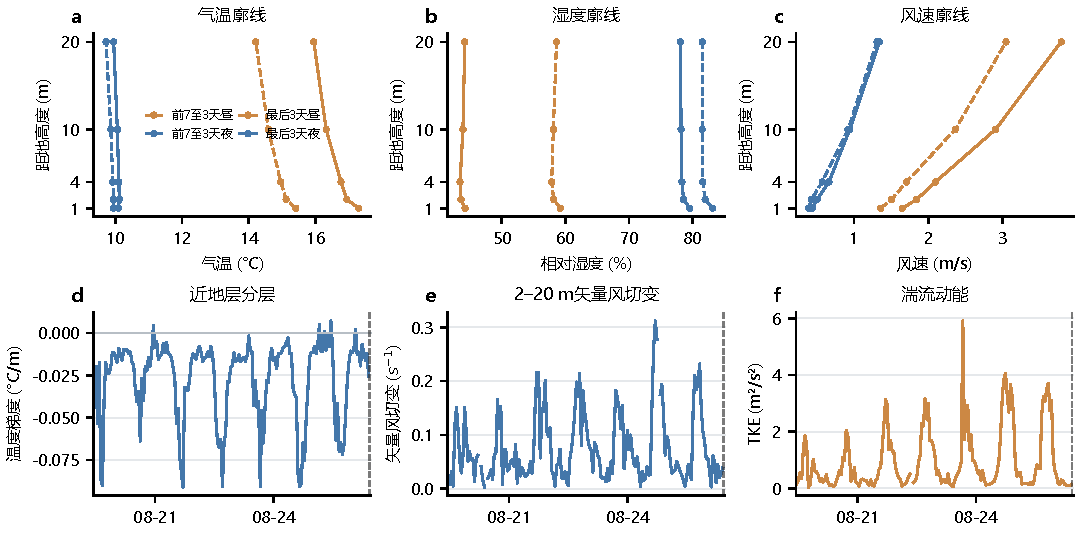
\includegraphics[width=\linewidth]{figures/fig3_1_boundary_layer.pdf}
\caption{多高度温湿风廓线与灾前分层、矢量风切变及湍动能。廓线虚/实线为前7至3天/最后3天；昼夜按固定钟点。时间轴为北京时间，竖线为题设参考，曲线不含灾后值。}\end{figure}
最后6h的$G_T$为-0.01519$^\circ$C/m，TKE为0.1378m$^2$/s$^2$，$u_*$为0.1304m/s，相对可用历史样本分别处在第26.5、24.9、40.2百分位，未显示该截点的极端湍流增强。2022年匹配FLUX缺测导致湍流组不能进入严格的五年组校准，但不影响本节对有效观测过程的描述。最后6h矢量风切变为0.0323s$^{-1}$，低于24h的0.0760s$^{-1}$；TKE也低于24h的1.183m$^2$/s$^2$。一周内TKE与风切变、$u_*$同步Spearman系数为0.76/0.87，与H/LE为0.62/0.57；含共同日周期，仅描述协变，不作因果或排名依据。20m塔只能反映本站近地层，不能代表源区冰崖或完整边界层。


\subsection{灾前天气过程与地气水热响应}
本站最后24h均温为13.74$^\circ$C，72h均温为13.23$^\circ$C，日变化明显且末期总体偏暖。相邻24h温差本站为0.442$^\circ$C，源区为-0.265$^\circ$C，短时温变并非完全同步。两地72h净辐射能分别为45.17和26.98MJ/m$^2$；源区24h潜热交换为68.20W/m$^2$。这些量描述热背景及地气交换，不能直接换算为冰体融化或失稳贡献。


\begin{figure}[H]\centering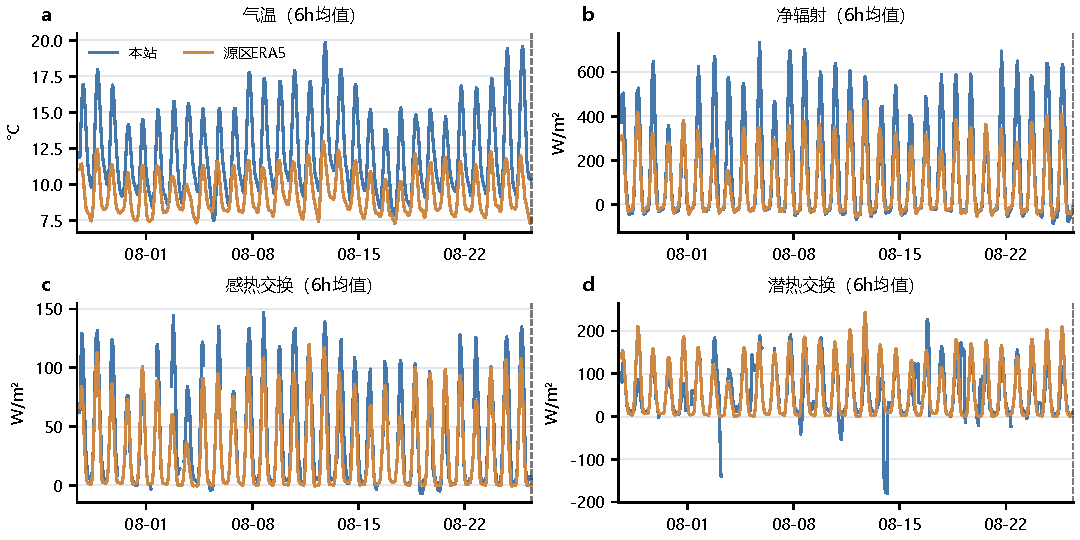
\includegraphics[width=\linewidth]{figures/fig3_2_energy_process.pdf}
\caption{灾前30天热状态与能量过程，作图为6h均值。本站保留供应通量符号，ERA5转换为向上正；未核实本站符号前，两地通量不作同向归因。}\end{figure}
本站前24/72h降水均为0，168h为3.8mm；源区ERA5分别为5.66、20.20、74.50mm。本站无雨不等于源区无水源。源区这三项处在历史第11.6、13.5、33.5百分位，本格点未见累计降水异常偏高，但不能排除未解析的局地天气。本站0.1m土壤湿度在一周内下降，末24h均值为0.08536m$^3$/m$^3$、24h变化为-0.01087m$^3$/m$^3$；深层变化更缓。这是本地陆面响应，不能替代冰川基底水压。


\begin{figure}[H]\centering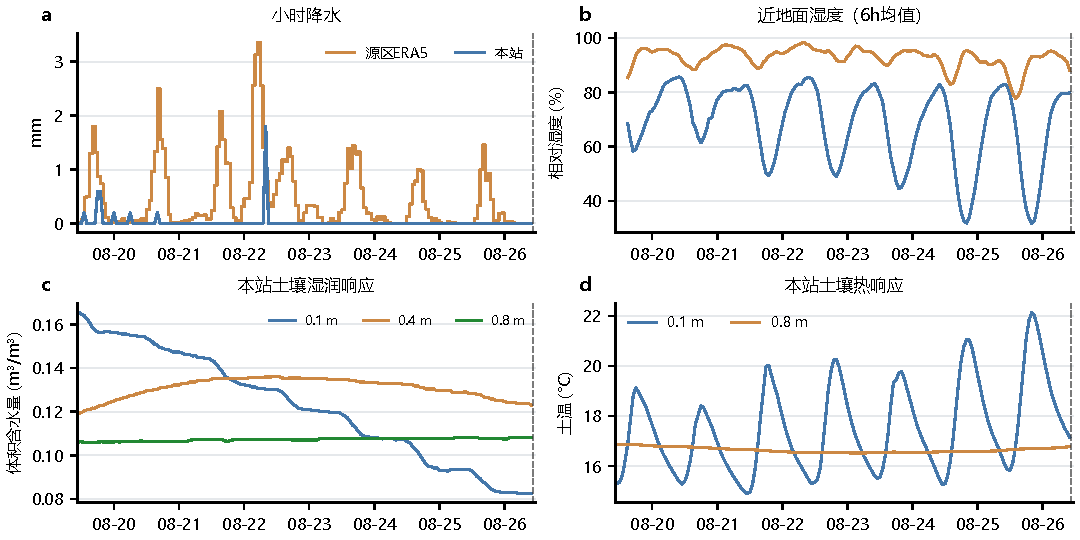
\includegraphics[width=\linewidth]{figures/fig3_3_water_process.pdf}
\caption{最后7天水分过程与本站土壤响应。源区与本站降水不同；土壤湿度、土温的深度差异不能外推成源区直接测量。}\end{figure}

\subsection{极端气象条件与历史异常识别}
在2021—2025年各取8月11日至9月10日同钟点，得到155个名义历史锚点；按实际有效数记录、年份等权。降水和风速采用预先规定的上尾，其余采用双侧经验尾部比例$r_j$，异常分数为$A_j=-\log_{10}r_j$。保留并列值与零值，经验比例不称独立样本p值。逐小时历史带匹配同季节同钟点，滚动窗口的超带时长只是持续性描述。
本站24h均温为第96.13百分位，浅层含水量24h变化为第3.87百分位，分别偏暖与偏干。最后7天两者超出历史5\%—95\%带分别为4h和115h；土壤变化最长连续超带60h。源区潜热和湿度为第87.10、13.55百分位，事件截点未超该区间；本站24h最大小时风速5.334m/s也仅约第38.7百分位。不能把全部环境异常混称极端天气，更不能预设暴雨或强风结论。


\begin{figure}[H]\centering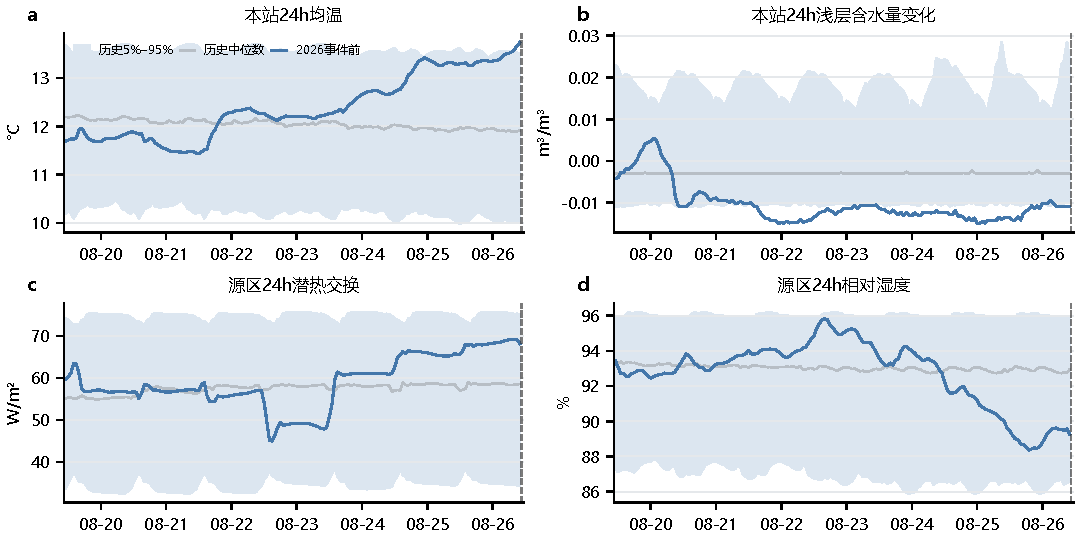
\includegraphics[width=\linewidth]{figures/fig3_4_historical_anomalies.pdf}
\caption{代表特征与历史同期中位数、5\%—95\%经验带。阴影不是预测/置信区间。可见本站干燥变化持续，源区潜热和湿度仍在历史波动范围内。}\end{figure}

\subsection{灾害关联证据评价与五因素筛选}
五个历史年按3年参照、2年校准作10种划分。每组取固定可用候选的最大异常$M_g=\max_j A_j$；历史校准也执行同样挑选，以校准尾部比例$Q_g$消除不同候选数的机会差异。每折真实与历史使用同一列全集。参照/校准每年至少15个有效锚点，不足则不可评估。各组中位$Q_g$越小，相对证据越强；至少60\%划分有效才能参加主前五。每组最多一个代表，跨组相关只作预先规定耦合组的冗余检查，不充当致灾关联。

\begin{table}[H]\centering\scriptsize
\caption{十组完整比较。历史百分位对应代表列，$Q$对应组内多版本校准后的中位比例；二者不等同。}
\begin{tabularx}{\linewidth}{llXrrrr}\toprule 组 & 因素 & 代表指标（站/源） & 事件前值 & 百分位 & $Q$ & 有效折\\\midrule
G8 & 土壤湿润 & 站 24h浅层含水量变化 & -0.011 & 3.9 & 0.230 & 10/10 \\
G1 & 温度状态与变化 & 站 24h平均气温 & 13.735 & 96.1 & 0.294 & 10/10 \\
G5 & 潜热交换 & 源 24h平均潜热通量 & 68.201 & 87.1 & 0.294 & 10/10 \\
G7 & 空气湿度 & 源 24h平均2m相对湿度 & 89.262 & 13.5 & 0.389 & 10/10 \\
G9 & 近地层热力分层 & 站 6h平均2至20m温度梯度 & -0.015 & 26.5 & 0.540 & 10/10 \\
G3 & 辐射条件 & 站 72h净辐射能量 & 45.170 & 89.4 & 0.600 & 10/10 \\
G4 & 感热交换 & 源 24h平均感热通量 & 34.618 & 69.7 & 0.635 & 10/10 \\
G6 & 风场 & 源 6h平均10m风速 & 0.603 & 67.1 & 0.758 & 10/10 \\
G2 & 前期降水 & 站 168h累计降水 & 3.800 & 41.0 & 0.881 & 10/10 \\
G10 & 湍流强度 & — & — & — & — & 0/10 \\
\bottomrule\end{tabularx}\end{table}

\begin{table}[H]\centering\scriptsize
\caption{最终五因素及证据边界。入选率的分母为22种同候选范围设置，不是独立灾害次数。}
\begin{tabularx}{\linewidth}{rlrlX}\toprule 排名 & 因素 & 代表值 & 设置入选率 & 解释边界\\\midrule
1 & 土壤湿润 & -0.01087 m$^3$/m$^3$ & 100.0\% & 本站干燥响应；非冰下水压 \\
2 & 温度状态与变化 & 13.74 $^\circ$C & 100.0\% & 区域偏暖；非融化量 \\
3 & 潜热交换 & 68.20 W/m$^2$ & 100.0\% & 模式地气交换；非实测融水 \\
4 & 空气湿度 & 89.26 \% & 100.0\% & 自身背景偏干；非因果 \\
5 & 近地层热力分层 & -0.01519 $^\circ$C/m & 72.7\% & 近地层代理；第5名较敏感 \\
\bottomrule\end{tabularx}\end{table}

相对前五为土壤湿润变化、温度状态与变化、潜热交换、空气湿度和近地层分层。G1/G5中位$Q$同为0.294，2/3次序只作展示，不宣称二者可精确区分。前四项在22种同范围设置均入选，第五项约72.7\%，部分设置由辐射或感热替代，故第五候选较弱。湍流无主排名源于2022年缺测；剔除该年的可用性结果仅作补充，不据此认定湍流无影响。


\begin{figure}[H]\centering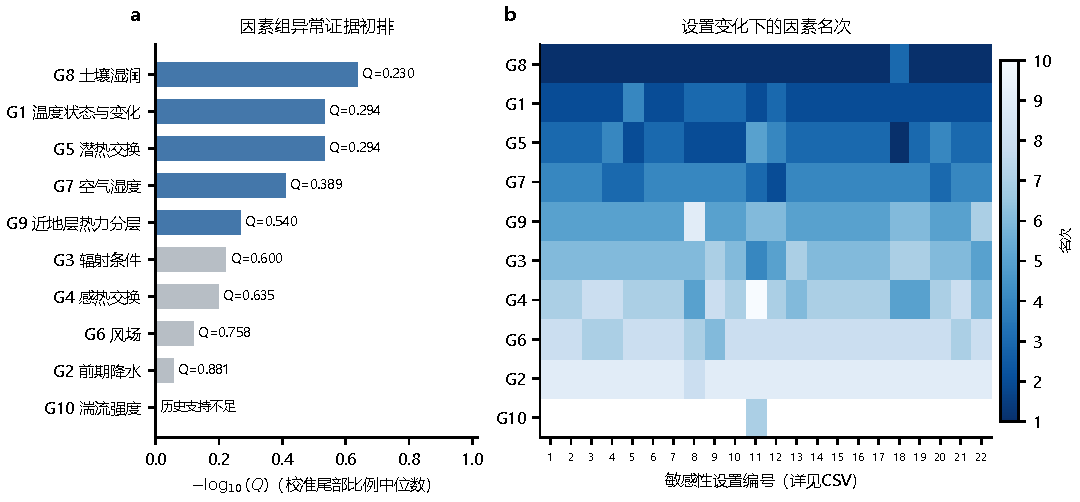
\includegraphics[width=\linewidth]{figures/fig3_5_ranking_stability.pdf}
\caption{组校准异常与设置稳健性。色阶为名次，灰白空格为不可评价；完整设置对应CSV。排名稳定不等于该因素具有因果贡献。}\end{figure}
进一步将历史校准期按7天留块并排除与168h窗口重叠部分，真实和伪事件在同一剩余校准集执行全套组筛选。620次相关比较中，有59.5\%的伪事件前五分数和不低于真实事件；同时五项中位$Q$均高于0.05。因此整体特殊性证据有限，不将五项升级为已证实的直接触发原因。本站土壤偏干只能解释当地陆面响应；区域偏暖不能直接推出源区融化，源区通量与湿度仅为格点环境背景。上述单事件相对排名可为后续研究提出候选，但不提供普适灾害发生概率。


\begin{thebibliography}{9}\small
\bibitem{Srivastava2022} Srivastava P, Namdev P, Singh P K. 7 February Chamoli Rock-Ice Avalanche Disaster: Model-Simulated Prevailing Meteorological Conditions. Atmosphere, 2022, 13:267. doi:10.3390/atmos13020267.
\bibitem{Zhong2025} Zhong Y, et al. Unravelling driving conditions of rock and ice avalanches and resulting cascading processes in High Mountain Asia. Landslides, 2025, 22:989--1001. doi:10.1007/s10346-024-02421-7.
\bibitem{ERA5} ECMWF. ERA5-Land data documentation and ARCO Product User Guide. Copernicus Knowledge Base. 累计规则与参数方向说明；数据源地址随项目附录交付。
\end{thebibliography}
